


\chapterauthor{Jeferson J. Lima}{Departamento de Informática (DAINF) \\Universidade Tecnológica Federal do Paraná (UTFPR)}
\chapter{Conceitos Básicos}


\section{Introdução}\label{intro}

A component part for an electronic item is
manufactured at one of three different factories, and then delivered to
the main assembly line.Of the total number supplied, factory A supplies
50\%, factory B 30\%, and factory C 20\%. Of the components
manufactured at factory A, 1\% are faulty and the corresponding
proportions for factories B and C are 4\% and 2\% respectively. A
component is picked at random from the assembly line. What is the
probability that it is faulty?

\section{Primeiros passos com a Linguagem Python}\label{python}

É comum quando estamos iniciando no mundo da matemática, nos depararmos com a necessidade de desenhar gráficos, algo como a figura baixo:

\begin{figure}
    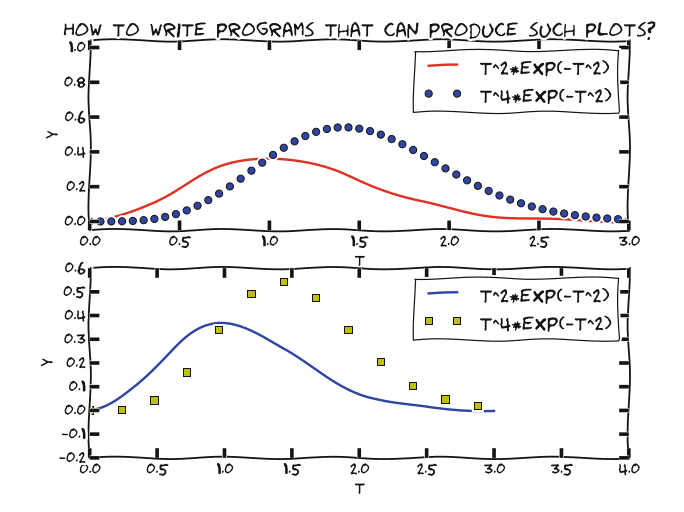
\includegraphics[width=250pt, height=200pt]{chapters/chapter0/figures/manual_graph.png}
    \caption[Desenhando Gráficos Manualmente]{Desenhando Gráficos Manualmente}
\end{figure}

Não somente nas engenharia os profissinais necessitam das habilidades de manipular e exibi-los dados graficamente, 
a maioria das pessoas tem experiencias em softwares como Microsoft Excel, Libreoffice Calc, entre outra ferramentas dedicadas.
No entanto, esse interação geralmente é bastante simples, com alguns cliques é possivel gerar diversos gráficos para visualização dos dados.

Porém, dada a caracteristica dos dados a serem plotados, faz-se necessário um nível de customização maior, surgindo a necessidade

Python é uma excelente linguagem para iniciantes, bem como usuários avançados, pois possui uma sintaxe simples e clara. Outro ponto
forte é as bibliotecas de python que apresenta diversas opções para processamento e visualização de dados. Destaca-se inicialmente aqui, duas
bibliotecas que serão utilizadas no inicialmente, a biblioteca para processamento numérico \textbf{numpy}, biblioteca \textbf{scipy} com diversas
funções da área de ciência da computação e  \textbf{matplotlib} para visualização dos dados.

\subsection{Instalação do Python}

Para estudar desta matéria, você precisa de uma instalação do Python que atenda ao propósito de aula. O mais rápido
maneira de obter uma instalação útil do Python em seu computador Windows ou Mac,
é baixar e instalar o Anaconda (https://www.anaconda.com/). Em muitas distribuições de linux, o Python já é nativo,
caso não seja, aconselha-se a instalação pelo terminal utilizando o comando
\begin{lstlisting}
    $ sudo apt-get install python3
\end{lstlisting}

A versão de Python2 está obsoleta desde janeiro de 2020, sendo assim, nem suporte desde então. Por este motivo aconselha-se
a instalação de Python3.

A instalação de uma biblioteca do Python pode ser dada através do comando:
\begin{lstlisting}
    $ sudo python3 -m pip install numpy
\end{lstlisting}

Há diversas opções de serviços online, como a ferramenta Colab do Google, onde disponibiliza opções com recursos computacionais interessantes,
a uma conta google são oferecidas três opções de hardware, Máquina sem GPU, com GPU e uma Máquina com TPU.

\subsection{Problemas Numéricos com Python}

Para o nosso primeiro exemplo de problema numérico utilizando a linguagem Python, vamos fazer uso da expressão do grafico xxx.

\begin{equation*}
    y = t^2\exp(-t^2)
\end{equation*}

Neste momento teremos que recorrer a algumas funções da biblioteca \textbf{numpy}, como \textbf{numpy.exp} e \textbf{numpy.linspace} para gerar um vetor de tempo $t$.

\begin{lstlisting}
    ## importando bibliotecas
    from numpy import exp, linspace
    ## Definindo a funcao
    def yf(t):
        return t**2*exp(-t**2)

    # vetor t, inicio em 0 e fim em 3
    #   com 50 elementos
    t = linspace(0,3,50)

    y = yf(t)
\end{lstlisting}

Assim a variável $y$ recebe $y_f(t)$.

\subsubsection{Plotando Dados}

Dando continuidade ao exemplo anterior, apresentamos aqui outra biblioteca do python, a  \textbf{matplotlib} para visualização dos dados.
Considerando o exemplo acima, temos:

\begin{lstlisting}
    ## importando bibliotecas
    from numpy import exp, linspace
    ## Definindo a funcao
    def yf(t,n):
        return t**n*exp(-t**2)

    # vetor t, inicio em 0 e fim em 3
    #   com 50 elementos
    t = linspace(0,3,50)

    y1 = yf(t,2)
    y2 = yf(t,4)

    # importando o modulo pyplot e renomeando como plt
    import matplotlib.pyplot as plt

    plt.plot(t,y1)
    plt.plot(t,y2, "o")
    plt.xlabel("t")
    plt.ylable("y")
    plt.legend(["T^2*EXP(-T^2)", "T^4*EXP(-T^2)"])
\end{lstlisting}

O resultado esperado será:

\begin{figure}[htb]
    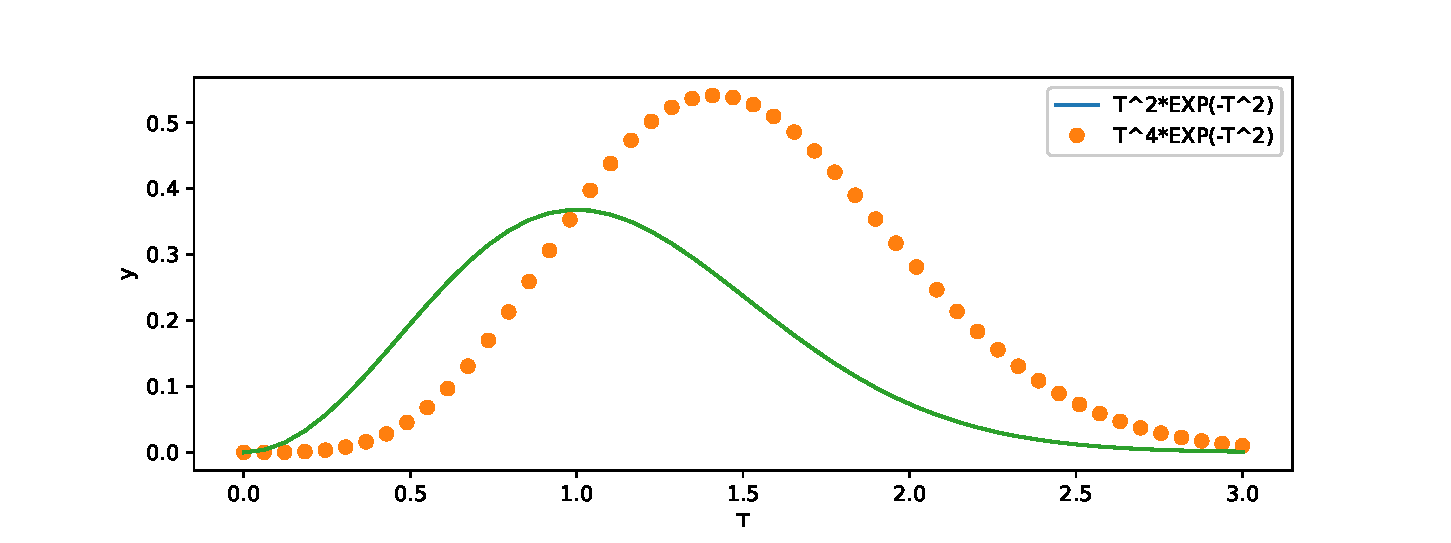
\includegraphics[width=300pt]{chapters/chapter0/figures/python_graph.eps}
    \caption[Desenhando Gráficos Manualmente]{Matplotlib Gráficos}
\end{figure}

A uma série de customizações que podem ser feitas no gráfico, como escrever a legenda em latex, mudança de cores, etc ... Para mais informações consulte a documentação do 
\textbf{matplotlib} na internet.

\subsubsection{Sistemas Dinâmicos}

\begin{VF}
    ``Um sistema dinâmico contínuo é um sistema dinâmico cujo estado evolui ao longo do espaço de estado continuamente de acordo com uma regra fixa.''
    
    \VA{Jaime E. Villate}{Introdução aos sistemas dinâmicos, 2007}
    \end{VF}

Para entender melhor como resolver numéricamente um sistema dinâmicos utilizando uma linguagem de programação, primeiro precisamos recorrer ao problema.

Aqui será apresentado um problema simples, onde deseja se saber a velocidade de um robô, considerando limitações impostas pelo seu modelo dînamico.
Considere um robô com rodas, onde numa superfície plana é aplicado uma força no sentido do seu movimento.

\begin{equation*}
    m\dot{v}+bv=u
\end{equation*}

Substituindo $v$ por $\dot{x}$:

\begin{equation*}
    m\ddot{x}+b\dot{x}=u
\end{equation*}

sendo $x$, posicionamento, $\dot{x}$ velocidade e $\ddot{x}$ aceleração, temos então a função de espaço de estados:

\begin{equation}\label{eq:car}
    \frac{d}{dt}\begin{bmatrix} x_0 \\ x_1 \end{bmatrix} = 
    \begin{bmatrix} 1 & 0\\ -\displaystyle\frac{b}{m} & +\displaystyle\frac{1}{m} \end{bmatrix}
    \begin{bmatrix} x_1 \\ u \end{bmatrix}    
\end{equation}

A solução numérica de Eq. \ref{eq:car} é obtida através de um método de integração, em Python a biblioteca \textbf{scipy} traz
os diversos métodos de integração, a função reponsável por chamar o integrador é \textbf{odeint}.

\begin{lstlisting}
    import numpy as np
    import matplotlib.pyplot as plt
    from scipy.integrate import odeint

    ## Definindo a funcao carro
    def car(x,t):
        m = 2000
        b = 240
        u = 100
        # inicializando vetor derivadas
        dx = np.zeros(2,)
        dx[0] = x[1]
        dx[1] = 1/m*(-b*x[1]+u)
        return dx

    # vetor t, inicio em 0 e fim em 3
    #   com 100 elementos
    t = np.linspace(0,10,100)
    # condicoes iniciais
    x0 = [0,0]

    # integrador
    x = odeint(car, x0, t)

    # plotando os valores
    plt.plot(t,x[:,0],t,x[:,1])
    plt.xlabel("t")
    plt.legend(["Posicao", "Velocidade"]) 
\end{lstlisting}
 
A solução numérica pode ser vista pelo gráfico abaixo:

\begin{figure}[htb]
    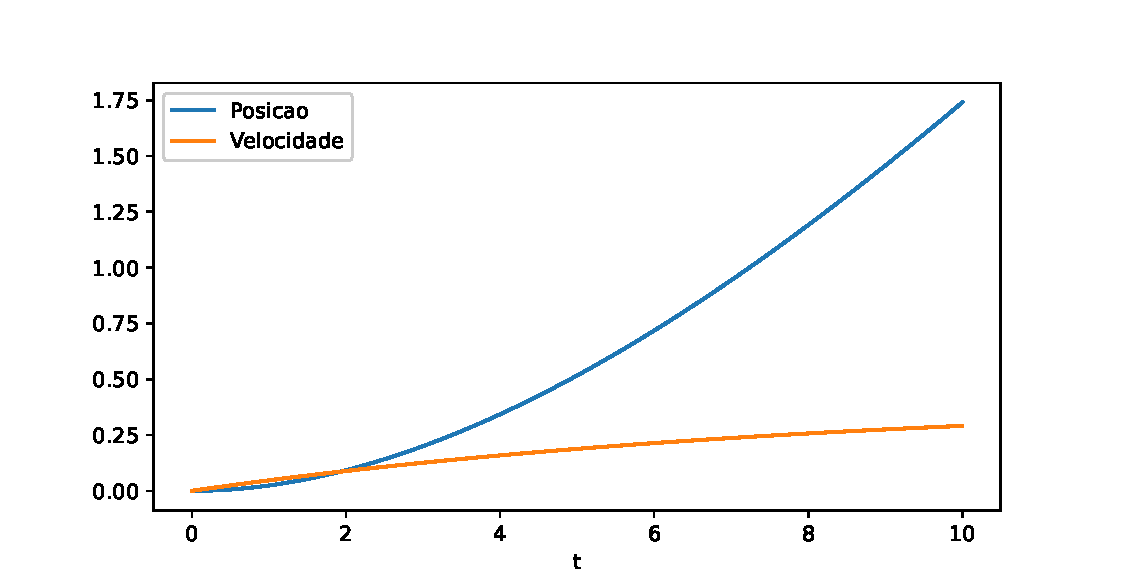
\includegraphics[width=300pt]{chapters/chapter0/figures/exercice_car.eps}
    \caption[Modelo Dinâmico Carro]{Gráfico velocidade e Posicionamento Carro}
\end{figure}

O sistema apresentado posui apenas dois estados, no entanto, sistemas de maior ordem podem ser 
simulados utilizando os métodos de integração, como será visto no próximo capítulo.


\section{Rotação, Translação e Transformação Homogênea}\label{rotacao}
 
\section{Glossário}
\begin{Glossary}
\item[360 Degree Review] Performance review that includes feedback from superiors, peers, subordinates, and clients.
\item[Abnormal Variation] Changes in process performance that cannot be accounted for by typical day-to-day variation. Also referred to as
non-random variation.
\item[Acceptable Quality Level (AQL)] The minimum number of parts that must comply with quality standards, usually stated as a percentage.
\item[Activity] The tasks performed to change inputs into outputs.
\item[Adaptable] An adaptable process is designed to maintain effectiveness and efficiency as requirements change. The process is
deemed adaptable when there is agreement among suppliers, owners, and customers that the process will meet
requirements throughout the strategic period.
\end{Glossary}



